\documentclass[a4paper,11pt]{article}
\usepackage[utf8]{inputenc} % un package
\usepackage[francais]{babel} %active le mode francais
\usepackage[top=2cm , bottom=2cm , left=2cm , right=2cm]{geometry} %propriétés de notre page
\usepackage{amsmath} %liste de symboles et applications mathématiques
\usepackage{color} %Permet d'utiliser la couleur dans nos documents
\usepackage{listings} %Paquet de coloration syntaxique (langages)
\usepackage{hyperref} % Créer des liens et des signets 
\usepackage[babel=true]{csquotes} %permet les quotations (guillemets)
\usepackage{graphicx} %Importation d'image

% Informations du rapport
\title {Rapport \\ Travaux Pratiques Réseaux (Ethernet)}
\author {Quentin Tonneau - Adrien Lardenois}
\date{}
%Propriétés des liens
\hypersetup{
colorlinks=true, %colorise les liens  
urlcolor= blue, %couleur des hyperliens 
linkcolor= blue,%couleur des liens internes 
} 

\begin{document}
	\maketitle %insère l'en-tête du rapport
	\tableofcontents %insère la table des matières ATTENTION : Compiler deux fois en cas de changements
	\newpage % Nouvelle page
	
	
	
	
	
	
	\section{Introduction}
	Après avoir mis en réseau un parc de pc (cf rapport tp \no 1), nous nous intéressons maintenant à la communication entre ces derniers. En s'appuyant sur le cours de réseaux Ethernet et nos connaissances en langage C dans l'environnement Linux, nous allons concevoir une suite d'applications destinées à interagir avec les PC voisins. Une bibliothèque de création et d'envoi de trame, ainsi qu'un sniffeur de réseau (affiche l'ensemble des trames circulant au voisinage de notre matériel) nous sont fournis afin de franchir les couches non étudiées en classe (4,5,6 et 7).
	\subsection{Écouter le réseau}
	Avant de communiquer sur un réseau, il nous faut un certain nombre d'informations sur le matériel avec lequel on souhaite ``entrer en discussion'', c'est à dire :
	%liste à puce
	\begin{itemize}
		\item Le nombre de personnes présentes sur le réseau
		\item Leurs adresses
		\item Le protocole de communication
		\item La nature des messages (émetteur, destinataire, type de message)
	\end{itemize}
	Pour cela, nous concevons un programme qui filtre les trames circulant sur le réseau, en ne conservant que les trames de type 9000 dont nous sommes le destinataire, puis affiche le message en question,tout en dressant une liste de toutes les machines (adresses MAC\footnote{Media access control}) présentes sur le réseau. On pourrait associer ce programme à un module de conversation type IRC\footnote{Internet Relay Tchat}, qui n'affiche que les messages personnels ou à destination de l'ensemble des utilisateurs.
	\subsection{Envoyer un message}
	Après avoir pris connaissance du materiel voisin, nous écrivons une fonction d'envois de trame simple, ainsi qu'un algorithme d'envois en boucle d'un ``bonjour'' sur le réseau (broadcast). Le type choisi pour ces échange est toujours 9000, afin de pouvoir être facilement reçu par les autres groupes du projet. Nous construisons la trame nécéssaire, et l'envoyons à l'aide des bibliothèques fournies, et du programme write\_eth\_frame.
	\subsection{Accusé la réception d'un message}
	L'unification des deux parties précédantes nous permet de programmer un répondeur automatique, qui en reçevant une trame de type 9000 sous la forme ``Bonjour de XX'' répond immédiatement à son emmeteur ``Bonjour de XX : bien reçu par Quentin et Adrien'', accusant ainsi la réception du message. Nous ré-implémentons l'analyse de la première partie, ainsi que nos connaissances en matière de traitement de la langue pour détecter les messages qui nous destinés, et nous utilisons la fonction d'envois de trame crée en deuxième partie pour répondre aux messages.
	\section{Structure du projet}
	\subsection{Structure des trames}
	Avant de nous lancer dans l'écriture des algorithmes de ce projet, nous avons dù analyser les bibliothèques fournies, et définir la structure de notre projet. La structure d'une trame est imposée, sous la forme :
	\lstset{language=C}
	\begin{lstlisting}
	struct eth_frame {
	char adr_dest[6];
	char adr_send[6];
	char type[2];
	char data[1500 - 6 - 6 - 2];
	};
	\end{lstlisting}
	On remarque donc que notre trame sera définie par deux adresses (destinataire et emetteur) MAC au format hexadécimal ($ 6$ octets $\to 12$ caracteres), d'un type (même encodage), et de données, n'excedant pas $1500-6-6-2=1486$ caractères. Une structure étant allouée de manière contigüe en mémoire, l'accès à l'adresse de l'emetteur pourra se faire sous la forme trame$\to$adr\_send ou bien (char*)trame[6] .
	\subsection{Arborescence du projet}
	Afin de faciliter la compréhension du projet, l'archive fournie est organisée de la sorte :
	\begin{itemize}
	\item Un fichier de compilation (script sh) se trouve à la racine
	\item Les fichiers sources (.c et .h) utiles au projet sont dans un répertoire \textbf{src}
	\item Une fois compilés, les 5 programmes se trouves dans le repertoire \textbf{bin}
	\end{itemize}
		\renewcommand{\labelitemii}{+}
	Liste et description des fichiers :
	\begin{itemize}
	\item \textbf{compilation.sh} : Fichier de Compilation (voir partie suivante)
	\item \textcolor{blue}{src}
		\begin{itemize}
		\item \textbf{envoyer\_trame .c/.h} : Fichier source de l'envois de trame (bonjour)
		\item \textbf{eth\_lib .c/.h} : Bibliothèque d'utilisation du réseau fournie
		\item \textbf{fonctions .c/.h} : Bibliothèque de fonctions communes au trois principaux programmes
		\item \textbf{inet\_str.h} : Structures des trames, nécéssaire à la compilation de eth\_lib
		\item \textbf{recevoir\_trame .c/.h} : Programme d'affichage des trames circulant sur le réseau
		\item \textbf{reponse\_auto .c/.h} : Programme de réponse automatique aux messages recu (accusé de réception)
		\item \textbf{sniff.c} : Programme de sniffage du réseau (fourni)
		\item \textbf{write\_eth\_frame.c} : Programme permettant l'envois de la trame donnée en premier paramètre (fourni)
		\end{itemize}
	\item \textcolor{blue}{bin}
		\begin{itemize}
		\item \textbf{envois} : programme d'envois des bonjours
		\item \textbf{recevoir} : programme d'affichage des trames
		\item \textbf{reponse} : programme d'accusé de reception
		\item \textbf{sniff} : programme utilisé pour l'execution de recevoir et reponse
		\item \textbf{write\_eth\_frame} : programme appelé par envois et reponse
		\end{itemize}
	\end{itemize}
	\subsection{Compilation et mode d'emplois}
		\subsubsection{Définition des variables avant compilation}
		Afin de compiler les différents algorithmes selon nos besoins, quelques variables (DEFINE) sont à préciser au début de chaque fichier source. En voiçi la liste :
		\begin{itemize}
		\item envoyer\_trame.c
			\begin{itemize}
			\item NOMBRE\_ENVOIS 200 \textit{Nombre de messages à envoyer}
			\item TEMPS\_ATTENTE 0    \textit{Temps entre deux envois (seconde)}
			\item ADRESSE ``e0:cb:4e:2f:fc:98" \textit{Adresse par défaut de la machine}
			\item MESSAGE``Bonjour de Quentin et Adrien" \textit{Message à envoyer}
			\end{itemize}
		\item recevoir\_trame.c
			\begin{itemize}
			\item TEMPS\_AFFICHAGE 50 \textit{Nombre de trame avant affichage de la liste}
			\end{itemize}
		\item reponse\_auto.c
			\begin{itemize}
			\item ADRESSE ``e0:cb:4e:2f:fc:98" \textit{Adresse par défaut de la machine}
			\end{itemize}
		\end{itemize}
		\subsubsection{Compilation}
		Pour compiler l'ensemble du projet, il suffit d'executer le fichier \textbf{compilation.sh}
		
		Si la compilation échoue, ou pour une architechture spécifique, voiçi les étapes de la compilation :
		\lstset{language=bash}
		\begin{lstlisting}
	#Cree le repertoire des programmes compiles
	mkdir bin
	#Compile la bibliotheque fournie (necessite inet_str.h)
	gcc src/eth_lib.c -c
	#Compile le logiciel d'envois de trame
	gcc src/write_eth_frame.c eth_lib.o -o bin/write_eth_frame
	#Compile le sniffeur
	gcc src/sniff.c eth_lib.o -o bin/sniff
	#Compile le programme d'envois
	gcc src/envoyer_trame.c eth_lib.o src/fonctions.c -o bin/envois
	#Compile le programme d'affichage
	gcc src/recevoir_trame.c eth_lib.o src/fonctions.c -o bin/recevoir
	#Compile le programme de reponse auto
	gcc src/reponse_auto.c eth_lib.o src/fonctions.c -o bin/reponse
	#Supprime le fichier de bibliotheque genere
	rm eth_lib.o
		\end{lstlisting}
		\subsubsection{Notes de compilation}
		Les éventuelles érreures dues à la compilation proviennent des bibliothèques et structures fournies par l'enseignant, mais n'impactent aucunement sur le fonctionnement des différents programmes générés. On remarque également que lors de la compilation du sniffeur sur des machines en environnement ``Ubuntu 11.04 et ultérieur version 32bits'' provoque des érreurs lors de l'execution (segmentation fault). Il est donc conseillé en cas d'erreur de compilation de reprendre les executables générés dans l'archive du projet, ou de contacter les auteurs des sources.
		\subsection{Manuel d'Instruction}
		Les programmes d'envois de trame (reponse et envois) prennent en paramètre l'adresse MAC\footnote{Les lettres doivent y figurer en minuscule} de la machine. Par défaut, l'adresse prise sera l'adresse indiquée dans les sources avant compilation (cf partie ci-dessus). Les programme de réception et d'analyse de trame (reponse et recevoir) doivent posseder en entrée la sortie standard de sniff au moyen d'un ``pipe'' ($|$).\\
		Selon les besoins, voici la liste des commandes d'éxecution :
		\begin{itemize}
		\item \textbf{bin/sniff $|$ bin/recevoir} : Affichage des trames (9000) qui circulent sur le réseau
		\item \textbf{bin/sniff $|$ bin/reponse ADRESSEMAC} : Affiche les messages qui nous sont destinés et répond automatiquement
		\item \textbf{bin/envois ADRESSEMAC} :		 Envois une série de trame dans un interval de temps (cf partie 2)
		\end{itemize}
		\subsection{Exemple de disposition}
		Pour utiliser pleinement les fonctions de ce projet, il faut donc ouvrir et disposer trois terminaux. Voiçi un exemple obtenu en placant l'afficheur en haut de l'écran, et les autres programmes en bas :\\
		\begin{center}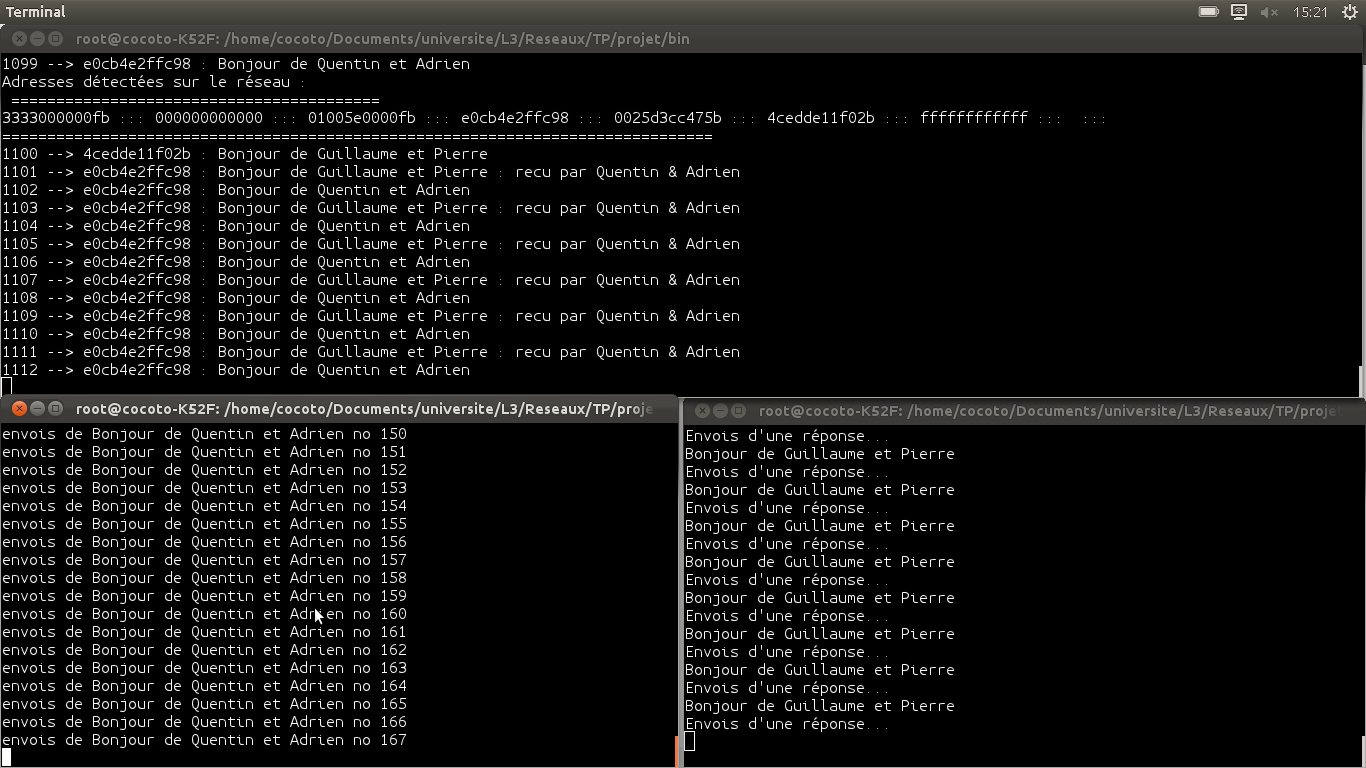
\includegraphics[width=15cm]{capture_ecran_rapport.png}\end{center}
	\section{Réception des trames}
	La reception de trames se fait par redirection de la sortie du sniffer vers notre programme défini par \textbf{recevoir\_trame.c}, au moyen d'un pipeline.
	Les informations reçues sont traitées une à une par la fonction \textit{lire\_trame()}. On vérifie alors si l'adresse de destination et l'adresse source nous sont déjà connus puis, si l'un et/ou l'autre est ``nouveau'', on l'ajoute à notre liste des matériels connectés.

	Nous avons choisi de représenter la liste des adresses rencontrées par une liste chainée. Cela a pour avantage de permettre l'ajout d'un maillon sans connaitre la taille actuelle de la liste, au contraire d'un tableau qu'il aurai fallu redimensionner au fur et à mesure.
	
	Dans un second temps, on vérifie si la trame appartient au type défini spécialement pour le TP (9000). Si c'est le cas, on affiche à l'écran les informations suivantes :
	\begin{itemize}
		\item Numéro de la trame (au moyen d'un compteur)
		\item Adresse source
		\item Contenu de la trame
	\end{itemize}

	Enfin, chaque fois que Y trames ont été affichées \footnote{Y étant défini au début du programme}, on affiche un récapitulatif des adresses qui circulent sur le réseau. Suivant le choix de Y (50 dans nos exemples) et en fonction du traffic sur le reseau, on beneficie alors d'un affichage clair des trames qui circulent avec un bilan regulier des utilisateurs presents. %d'ailleurs on pourrai de temps en temps vider la liste pour se debarasser des utilisateurs inactifs sur le reseau depuis trop longtemps.
	\subsection{la fonction lire\_trame}
	La fonction \textit{lire\_trame} est définie dans \textbf{fonctions.c}. Elle retire les 3 premiers caractères de la sortie du sniffer qui ne nous intéressent pas, puis récupère la longueur de la trame. Apres quoi elle capte toute la trame grâce à la fonction \textit{get\_buf} et la retourne en sortie.
	\subsection{la fonction recherche}
	La fonction \textit{ recherche} parcoure la liste chainée à partir du premier maillon et s'arrête si en passant au suivant elle arrive à NULL. Il est possible de faire le test à la fin car l'initialisation de la liste garanti l'existence d'au moins un maillon different de NULL.

	Pour chaque maillon, on compare le champ adresse à celle que l'on cherche : s'il y a correspondance on sort directement en renvoyant 1, sinon on passe au suivant. Si la recherche a eu lieu jusqu'au bout sans succes, on retourne 0.
	\subsection{la fonction ajout}
	La fonction d'ajout ajoute un élément en tete de liste. On crée simplement un nouvel élément que l'on défini comme l'adresse à ajouter et dont le suivant est l'ancienne tete de liste.
	\subsection{la fonction affiche}
	La fonction  \textit{affiche} parcoure la liste de la même maniere que  \textit{recherche} . Pour chaque étape de la liste, elle affiche l'adresse et separe les adresses par :::
	\section{Envois des trames (type 9000)}
	\subsection{Fonction d'envois}
	Maintenant que nous recevons les trames de type 9000, nous devons à notre tour envoyer, afin de :
	\begin{itemize}
	\item Nous identifier sur le réseau
	\item Échanger des informations
	\item Accuser la réception d'informations externes
	\end{itemize}
	Pour celà, une fonction nommée ``envois\_trame'' dans le fichier fonctions.c construit la trame en fonctions des paramètres :
	\lstset{language=C}
\begin{lstlisting}
//Envois une trame sur le reseau, de type 9000
void envois_trame(char *source, char *dest, char *message)
\end{lstlisting}
	où source et dest sont les adresses MAC des machines concernées au format XX:XX:XX:XX:XX:XX. Pour celà, nous avons créé une procédure convaddr qui converti les adresses en ajoutant le caractère \enquote{:}. Ensuite, nous créeons la trame à l'aide de la fonction
	\lstset{language=C}
\begin{lstlisting}
int make_ping_request(char* eth_addr_dest, char* eth_addr_send,
 char* type_frame, char* data, struct eth_frame* frame);
\end{lstlisting}
	dont la valeur de retour nous indique la taille de la trame générée. Nous convertissons ensuite cette trame au format hexadécimal par la fonction char\_to\_charhexa et nous envoyons la trame en passant cette dernière en paramètre du programme write\_eth\_frame fourni dans le projet.
	\subsection{Programme de présentation}
	Afin de nous présenter une fois connecté sur le réseau, nous avons créé le programme \textit{recevoir\_trame.c} dont les paramètres suivants sont à définir avant la compilation :
	\lstset{language=C}
\begin{lstlisting}
#define NOMBRE_ENVOIS 10  //Nombre de message a envoyer
#define TEMPS_ATTENTE 1	  //Temps d'attente entre deux envois (secondes)
#define ADRESSE "e0:cb:4e:2f:fc:98" //Adresse par defaut
#define MESSAGE "Bonjour de Quentin et Adrien" //Message
\end{lstlisting}
	Ce programme envois un certain nombre de fois un message d'identification sur le réseau, à l'adresse de broadcast \textit{ff:ff:ff:ff:ff:ff}.
	
	
	
	
	\section{Synthèse et automatisation}
	\section{Bilan}
\end{document}
